\documentclass[10pt]{scrartcl}

\usepackage[T1]{fontenc}
\usepackage{amssymb, amsmath, amsthm}
\usepackage{geometry, graphicx, enumitem, wrapfig, fancyhdr,cancel}
\usepackage{listings, xcolor}
\usepackage[english]{babel}

\definecolor{codegreen}{rgb}{0,0.6,0}
\definecolor{codegray}{rgb}{0.5,0.5,0.5}
\definecolor{codepurple}{rgb}{0.58,0,0.82}
\definecolor{backcolour}{rgb}{0.95,0.95,0.92}

\lstdefinestyle{mystyle}{
    backgroundcolor=\color{backcolour},   
    commentstyle=\color{codegreen},
    keywordstyle=\color{magenta},
    numberstyle=\tiny\color{codegray},
    stringstyle=\color{codepurple},
    basicstyle=\ttfamily\footnotesize,
    breakatwhitespace=false,         
    breaklines=true,                 
    captionpos=b,                    
    keepspaces=true,                 
    numbers=left,                    
    numbersep=5pt,                  
    showspaces=false,                
    showstringspaces=false,
    showtabs=false,                  
    tabsize=4
}
\lstset{style=mystyle}
\geometry{a4paper, margin=0.8in}
\pagestyle{fancy}
\lhead{PH2101 - Assignment 04 Solutions}
\rhead{Debayan Sarkar \texttt{22MS002}}
\everymath{\displaystyle}
\theoremstyle{definition}
\newtheorem{exercise}{Question}
\newenvironment{solution} {\begin{proof}[\normalfont \textbf{Solution}]} {\end{proof}}

\renewcommand{\qedsymbol}{}
\newcommand{\nn}{\mathbb{N}}
\newcommand{\npixL}{\frac{n\pi x}{L}}
\newcommand{\rn}{\mathbb{R}}
\newcommand{\q}{\mathbb{Q}}
\newcommand{\p}{\mathcal{P}}
\newcommand{\z}{\mathbb{Z}}
\newcommand{\dx}{\mathrm{d}x}
\usepackage{mlmodern}
\title{PH2101 - Waves and Optics}  
\subtitle{Assignment 4 Solutions}
\author{Debayan Sarkar \\ \texttt{22MS002}}
\date{\today}

\geometry{a4paper, margin=1in}
\setlength{\parindent}{0pt}
\begin{document}
\maketitle
\begin{exercise}
    Consider a one-dimensional oscillator of unit mass and of natural frequency $\omega_0$ (natural fre-
    quency: frequency of undamped oscillation). The oscillator experiences a velocity dependent
    damping with a damping coefficient $\gamma$.
    Initially the oscillator was at rest $x(0) = \dot{x}(0) = 0$. The oscillator is subjected to a force given
    by $F_0\cos \omega t$.
    \begin{enumerate}[label={(\alph*)}]
        \item Find the complete solution as a function of time.
        \item Check the case when the driving frequency is equal to the natural frequency.
    \end{enumerate}
    \begin{solution}
        $ $
        \begin{enumerate}[label={(\alph*)}]
            \item The differential equation for the given system will be, 
                $$\ddot{x} +\frac{\gamma}{m} \dot{x}+ \omega_0^2x = \frac{F_0}{m} \cos\omega t$$
                Let $\alpha := \frac{\gamma}{m}$.
                First we solve the homogenous part of this equation by assuming, $x = Ae^{i\omega't}$.
                Then, we have
                \begin{align*}
                    & -\omega'^2 + i\alpha \omega' + \omega_0^2 = 0 \\ 
                    \Rightarrow & \omega'^2 - i\alpha \omega' - \omega_0^2 = 0 \\ 
                    \Rightarrow & \omega' = \frac{i\alpha \pm \sqrt{4\omega_0^2 - \alpha^2}}{2}\\ 
                    \Rightarrow & \omega' = \frac{i\alpha}{2} \pm \sqrt{\omega_0^2 - \frac{\alpha^2}{4}}
                \end{align*}
                Let $\omega_1 = \sqrt{\omega_0^2 - \frac{\alpha^2}{4}}$. Then, the solution to the homogemous solution is, 
                \begin{align*}
                    x &= Ae^{i({\frac{i\alpha}{2} + \omega_1})t}+ Be^{i({\frac{i\alpha}{2} - \omega_1})t} \\ 
                      &= e^{-\frac{\alpha t}{2}}(Ae^{i\omega_1t} + Be^{-i\omega_1t}) \\ 
                      &= e^{-\frac{\alpha t}{2}}(C\cos\omega_1t + D\sin\omega_1t)
                \end{align*}

                Since the RHS is $\frac{F_0}{m}\cos\omega t$, we take a guess that $x(t)$ is of the form $x = Ae^{i\omega t}$.
                Then, putting this value in the equation we get, 
                \begin{align*}
                    &A[-\omega^2 -i\alpha \omega + \omega_0^2] = \frac{F_0}{m} \\ 
                    \Rightarrow &A = \frac{F_0}{m} \cdot \frac{1}{i\alpha\omega + (\omega_0^2 - \omega^2)} \\ 
                    \Rightarrow &A = \frac{F_0}{m} \cdot \frac{1}{\sqrt{\alpha^2\omega^2 + (\omega_0^2 - \omega^2)^2} e^{i\phi}}
                \end{align*}
                Where $\phi = \arctan{\left(\frac{\alpha \omega }{\omega_0^2 - \omega^2}\right)}$
                Hence, the solution is
                $$\boxed{x(t) =e^{-\frac{\alpha t}{2}}(C\cos\omega_1t + D\sin\omega_1t) + A\cos{\left(\omega t - \phi\right)}}$$
                Putting the initial values in the problem we get, $\boxed{C = -A\cos\phi}$ and 
                \begin{align*}
                    &-\frac{\alpha}{2}C + \omega_1 D + \omega A \sin \phi = 0 \\ 
                    \Rightarrow &\omega_1D = -A\left(\omega\sin\phi + \frac{\alpha}{2}\cos\phi\right) \\ 
                    \Rightarrow &\boxed{D = -\frac{A}{\omega_1}\left(\omega\sin\phi + \frac{\alpha}{2}\cos\phi\right)}
                \end{align*}
                This determines $x(t)$ uniquely.
            \item When driving frequency is equal to the natural frequency, we have $\omega = \omega_0$. Clearly, in this case, the amplitude of oscillation is maximum. The particular solution will be, 
                $$\boxed{x(t) = \frac{F_0}{m \alpha \omega} e^{i(\omega t - \frac{\pi}{2})}}$$
                Since, $\phi = \arctan{\frac{\alpha \omega}{\omega_0^2 - \omega^2}}=\frac{\pi}{2}$ and $A = \frac{F_0}{m\alpha\omega}$. So, if we want to write the same solution,
                the values of $C$ and $D$ will be, $\boxed{C = 0}$ and $\boxed{D = -\frac{A\omega}{\omega_1}}$
            \end{enumerate}
    \end{solution}
    \begin{exercise}
        Consider how to solve the steady-state motion of a forced oscillator if the driving force is of 
        the form $F = F_0 \sin \omega t$ instead of $F_0 \cos \omega t$.
    \end{exercise}
    \begin{solution}
        If it's $\sin$ instead of $\cos$, we solve it the exact similar way, except when solving for the particular solution, we
        put $-i \frac{F_0}{m}$ in the RHS, since we are working with the Sine part of the complex exponential.

        Hence, after solving we obtain the particular solution to be $x(t) = A \sin \left(\omega t - \phi\right)$

        After that we again proceed similarly to determine the constants $C$ and $D$ from the homogenous part.
    \end{solution}
    \begin{exercise}
        A block of mass $m$ is connected to a spring, the other end of which is fixed. There is also a
        viscous damping mechanism. The following observations have been made on this system:
        \begin{enumerate}
            \item If the block is pushed horizontally with a force equal to $mg$, the static compression of the spring is equal to $h$.
            \item The viscous resistive force is equal to $mg$ if the block moves with a certain known speed $u$.
        \end{enumerate}
        \begin{enumerate}[label = {(\alph*)}]
            \item For this complete system (including both spring and damper) write the differential equation governing horizontal oscillations of the mass in terms of $m$, $g$, $h$, and $u$.
            Answer the following for the case that $u = 3\sqrt{gh}$.
            \item What is the angular frequency of the damped oscillations?
            \item After what time, expressed as a multiple of $\sqrt{h/g}$, is the energy down by a factor $1/e$?
            \item What is the quality factor $Q$ of this oscillator?
            \item  This oscillator, initially in its rest position, is suddenly set into motion at $t = 0$ by a bullet
            of negligible mass but nonnegligible momentum traveling in the positive $x$ direction. Find
            the value of the phase angle $\phi$ in the equation $x = Ae^{-\frac{\alpha t}{2}} \cos(\omega t - \phi)$ that describes the
            subsequent motion, and sketch $x$ versus $t$ for the first few cycles.
            \item If the oscillator is driven with a force $mg \cos \omega t$, where $\omega = \sqrt{2g/h}$, what is the amplitude
            of the steady-state response?
        \end{enumerate}
    \end{exercise}
    \begin{solution}
        $ $
        \begin{enumerate}[label={(\alph*)}]
            \item From the given information about the system we can deduce that, 
                $$k = \frac{mg}{h} \text{ and } \gamma = \frac{mg}{u}$$
                Hence, the differential equation turns out to be as in Question 1, 
                $$\ddot{x} + \frac{g}{u}\dot{x} + \frac{g}{h} x = 0$$
                For $u = \sqrt{3gh}$ we get,
                $$\ddot{x} + \frac{1}{3}\sqrt{\frac{g}{h}}\dot{x} + \frac{g}{h} x = 0$$
            \item Let $x = Ae^{i\omega' t}$. Then, as previously done for the homogneous part in Question 1, 
                \begin{align*}
                    \omega' &= \frac{i}{6}\sqrt{\frac{g}{h}} \pm \sqrt{\frac{g}{h} - \frac{g}{36h}} \\ 
                            &= \frac{i}{6}\sqrt{\frac{g}{h}} \pm \sqrt{\frac{35g}{36h}}
                \end{align*}
                Let $\omega = \sqrt{\frac{35g}{36h}}$ and $\alpha = \sqrt{\frac{g}{9h}}$. Then, the solution of the equation turns out to be, 
                $$\boxed{x(t) = e^{-\frac{\alpha}{2} t}C\cos (\omega t - \phi)}$$
                Where the angular frequency ($\omega$) is given by, 
                $$\boxed{\omega = \sqrt{\frac{35g}{36h}}}$$
            \item We have 
                \begin{align*}
                    &\dot{x} = Ce^{-\frac{\alpha t}{2}}\cos(\omega t - \phi) \\ 
                    \Rightarrow &\dot{x} = -Ce^{-\frac{\alpha t}{2}}[\omega\sin(\omega t - \phi) + \frac{\alpha}{2}\cos(\omega t - \phi)] \\ 
                    \Rightarrow &\dot{x} = -Ce^{-\frac{\alpha t}{2}}\omega[\sin(\omega t - \phi) + \frac{\alpha}{2\omega}\cos(\omega t - \phi)] \\ 
                    \Rightarrow &\dot{x} \sim -Ce^{-\frac{\alpha t}{2}}\omega_0\sin(\omega t - \phi) \tag{$\omega_0 >> \alpha \Rightarrow \omega = \sqrt{\omega_0^2 - \frac{\alpha^2}{4}} \sim \omega_0$} 
                \end{align*}
                Total energy can be written as, 
                \begin{align*}
                    &E = \frac{1}{2}m\dot{x}^2 + \frac{1}{2}\frac{mg}{h}x^2 \\ 
                    \Rightarrow &E = \frac{mC^2g}{2h}e^{-\alpha t}
                \end{align*}
                We are given that, $E(t) = \frac{1}{e}E(0) \Rightarrow e^{-\alpha t} = \frac{1}{e} \Rightarrow t = \frac{1}{\alpha} = 3\sqrt{\frac{h}{g}}$

                Hence, it's $3$ units of $\sqrt{\frac{h}{g}}$.
            \item $Q = \frac{\omega_0}{\gamma} = \sqrt{\frac{g}{h}} \cdot 3\sqrt{\frac{h}{g}} = 3$
            \item  According to the given conditions, we have $x = 0$ and $\dot{x} \neq 0$. Then, putting these values
                we get $\boxed{\phi = \frac{\pi}{2}}$ Hence, the solution is 
                $$\boxed{x(t) = Ae^{-\frac{\alpha t}{2}}\sin\omega t}$$
                \begin{figure}[h]
                    \centering
                    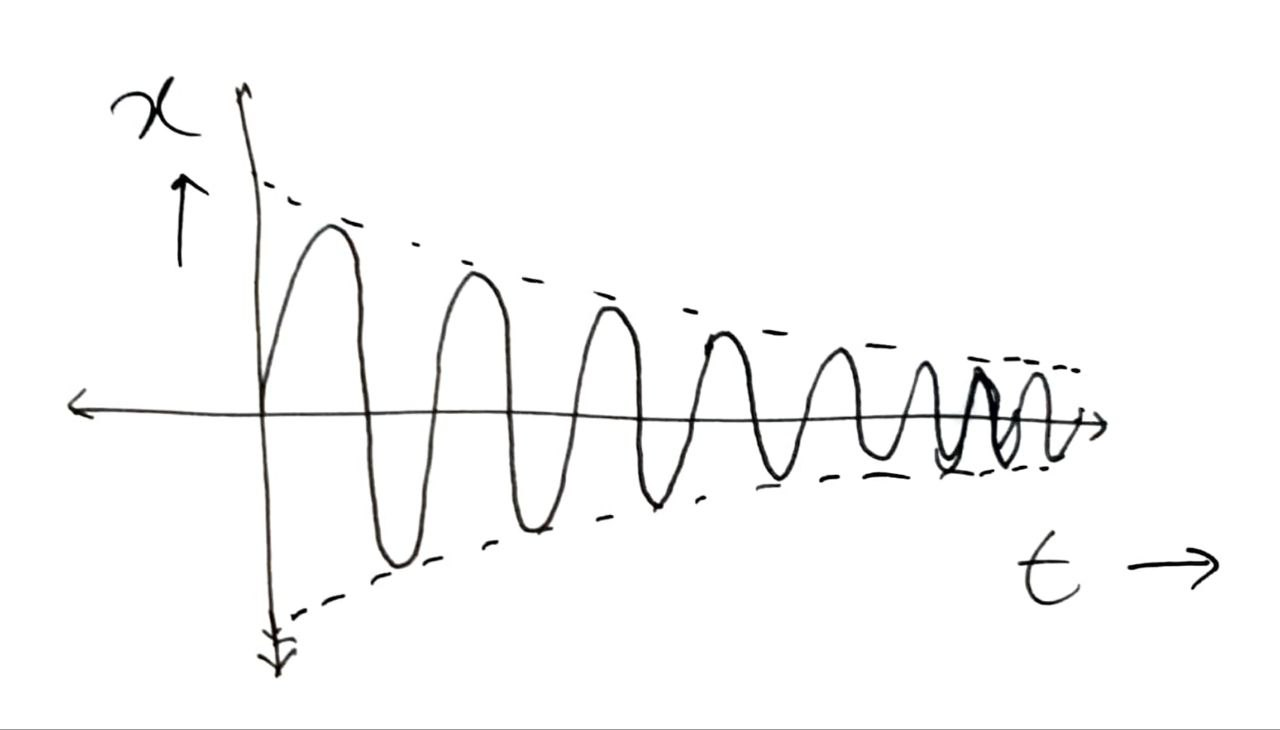
\includegraphics[width = 4.0in]{damped.jpg}
                \end{figure}
            \item The amplitude of the steady state response can be obtained as:
                \begin{align*}
                    &A = \frac{F_0}{m} \frac{1}{\sqrt{\alpha^2\omega^2 + (\omega_0^2 - \omega^2)^2}} \\ 
                    \Rightarrow &A = \frac{g}{\sqrt{\frac{g}{9h}\cdot \frac{2g}{h} + (\frac{g}{h} - \frac{2g}{h})^2}} \\ 
                    \Rightarrow &A = \frac{h}{\sqrt{1 + \frac{2}{9}}} \\ 
                    \Rightarrow &\boxed{A = \frac{3h}{\sqrt{11}}}
                \end{align*}
        \end{enumerate}
    \end{solution}
\end{exercise}
\end{document}

